\documentclass{article}
\usepackage{graphicx}
\usepackage{xcolor}
\usepackage{array}
\usepackage[T1]{fontenc}
\usepackage{bbding}
\usepackage{amsfonts}
\usepackage{amsmath}
\usepackage{pgfgantt}
\usepackage[margin=2cm]{geometry}
\usepackage[hidelinks]{hyperref}
\usepackage{subcaption}
\usepackage{float}
\usepackage{verbatim}
\usepackage{setspace}
\usepackage{titling}
\newcommand\Tstrut{\rule{0pt}{2.6ex}}
\newcommand\Bstrut{\rule[-0.9ex]{0pt}{0pt}}
\newcommand{\TBstrut}{\Tstrut\Bstrut}
\renewcommand{\contentsname}{Sommaire}
\newcommand{\stepimage}[3][0.3\textwidth]{%
  \minipage{#1}
    \includegraphics[width=\linewidth]{ressources/#2}
    \caption{#3}
  \endminipage\hfill
}

\title{\vspace{-3.0cm}
\rule{0.65\linewidth}{3pt}\\[0.7em]  % Upper line, 2pt thick
OCR Word Search Solver\\[0.5em]
\rule{0.65\linewidth}{1pt}           % Lower line, 1pt thick
}

\author{
    \begin{tabular}{cc}
        \small\textbf{Alexandre Joaquim Lima Salgueiro} & \small\textbf{Hugo Guyennet} \\
        \small\texttt{alexandre-joaquim.lima-salgueiro} & \small\texttt{hugo.guyennet} \\[2ex]
        \small\textbf{Léa-Angélina Kolmerschlag} & \small\textbf{Tom Huynh} \\
        \small\texttt{lea-angelina.kolmerschlag} & \small\texttt{tom.huynh}
    \end{tabular}
}


\date{4 novembre 2025}

\begin{document}

\maketitle

\begin{spacing}{0.9}
\tableofcontents
\end{spacing}



\section{Rôle et mission de chaque membre}

\begin{itemize}
    \item \textbf{Chargement des images et mise à l'échelle de gris :} Léa-Angélina Kolmerschlag
    \item \textbf{Rotation de l'image :} Léa-Angélina Kolmerschlag
    \item \textbf{Pré-traitement de l'image :} Tom Huynh
    \item \textbf{Extraction de la grille et des cellules :} Tom Huynh
    \item \textbf{Extraction des mots :} Tom Huynh et Alexandre Joaquim Lima Salgueiro
    \item \textbf{Réseau de neurones :} Tom Huynh et Hugo Guyennet
    \item \textbf{Solver :} Alexandre Joaquim Lima Salgueiro
\end{itemize}

\section{Objectifs, planification et état d'avancement}

\subsection{Objectifs du projet}
L'objectif principal du projet était de concevoir et d'implémenter un système complet capable de résoudre des grilles de mots mêlés à partir d'une simple image.

\subsubsection*{Éléments pour la première soutenance}
\begin{itemize}
    \item[\Checkmark] Chargement d’une image et suppression des couleurs ;
    \item[\Checkmark] Rotation manuelle de l’image ;
    \item[\Checkmark] Détection de la position :
    \begin{itemize}
        \item De la grille ;
        \item De la liste de mots ;
        \item Des lettres dans la grille ;
        \item Des mots de la liste ;
        \item Des lettres dans les mots de la liste.
    \end{itemize}
    \item[\Checkmark] Découpage de l’image (sauvegarde de chaque lettre sous la forme d’une image) ;
    \item[\Checkmark] Implémentation de l’algorithme de résolution d’une grille de mots cachés dans le programme en ligne de commande \texttt{solver} ;
    \item[\Checkmark] Une preuve de concept du réseau de neurones, capable d’apprendre la fonction logique XNOR.
\end{itemize}

\subsubsection*{Éléments pour la soutenance finale}
\begin{itemize}
    \item[\PencilRight] Le prétraitement complet (avec la rotation automatique) ;
    \item[\PencilRight] Le réseau de neurones complet et fonctionnel :
    \begin{itemize}
        \item Apprentissage ;
        \item Reconnaissance des lettres de la grille et de la liste de mots.
    \end{itemize}
    \item[\Checkmark] La reconstruction de la grille ;
    \item[\Checkmark] La reconstruction de la liste de mots ;
    \item[\XSolidBrush] La résolution de la grille ;
    \item[\XSolidBrush] L’affichage de la grille ;
    \item[\XSolidBrush] La sauvegarde du résultat ;
    \item[\PencilRight] Une interface graphique permettant d’utiliser tous ces éléments.
\end{itemize}


\subsection{Planification et état d'avancement}
Le projet a été découpé en plusieurs phases successives, de la manipulation d'image basique à la résolution finale. Une planification initiale a été établie pour suivre la progression des différentes tâches.

Le projet respecte les délais prévus et présente même une avance sur la planification initiale. Le pipeline fonctionnel est capable de traiter avec succès les images de \textbf{niveau 3}, qui représentent les cas les plus complexes fournis (images bruitées, tournées, avec des conditions d'éclairage non-uniformes).
\subsection{Note sur la reconnaissance de caractères (OCR)}
Dans le cadre de ce projet, un réseau de neurones convolutionnel (CNN) a été développé en interne pour la reconnaissance optique des caractères (OCR). Ce réseau, bien que non présenté dans ce rapport, atteint une précision satisfaisante pour la reconnaissance des lettres dans les cellules extraites de la grille.

Le choix de ne pas détailler cette partie dans le présent rapport est motivé par la volonté de se concentrer sur les aspects de traitement d'image et d'analyse de structure, qui constituent le cœur de notre contribution. Le réseau XNOR présenté précédemment sert d'illustration des principes de base des réseaux de neurones, tandis que notre CNN d'OCR est une implémentation plus complexe et spécifique.

\newpage
\section{Extraction de la grille et des mots}
Le but de l'extraction de la grille et des mots et de pouvoir donner les informations extraites au solver. Ce processus peut être vu comme une application d'algorithme de computer vision \cite{szeliski2010computer}.

Nous prendrons comme exemples ces 3 images :

\begin{figure}[!htb]
    \minipage{0.30\textwidth}
      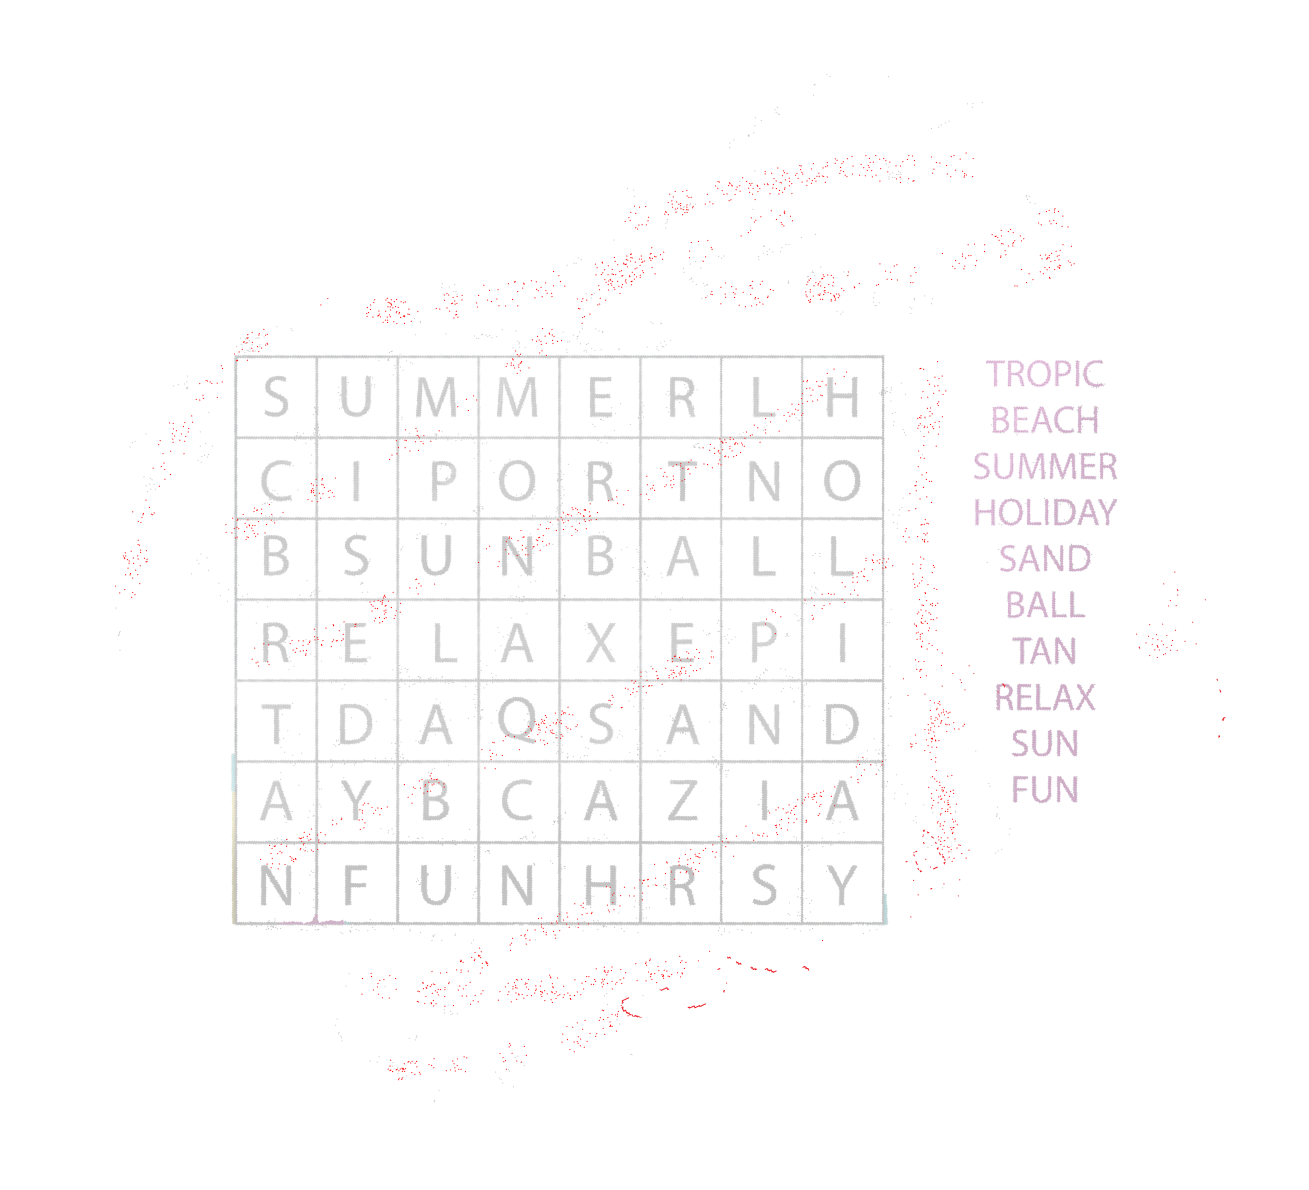
\includegraphics[width=\linewidth]{ressources/image_1.png}
      \caption{Grille avec du bruit et difficilement lisible}
    \endminipage\hfill
    \minipage{0.30\textwidth}
      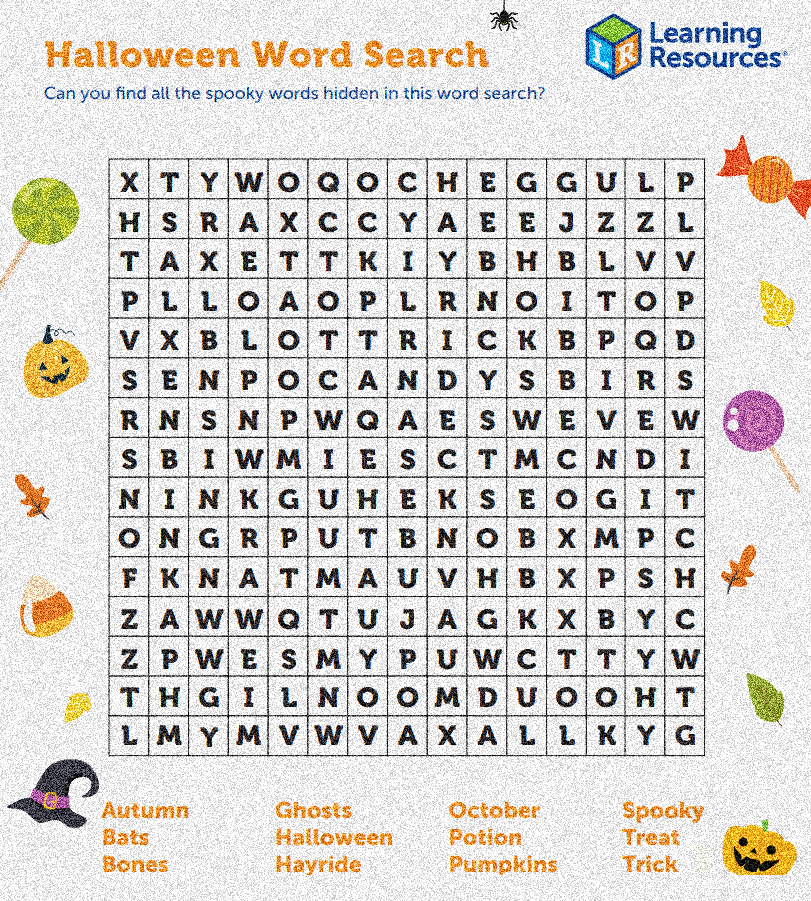
\includegraphics[width=\linewidth]{ressources/image_2.png}
      \caption{Grille avec des éléments autours et beaucoup de grain}
    \endminipage\hfill
    \minipage{0.26\textwidth}%
      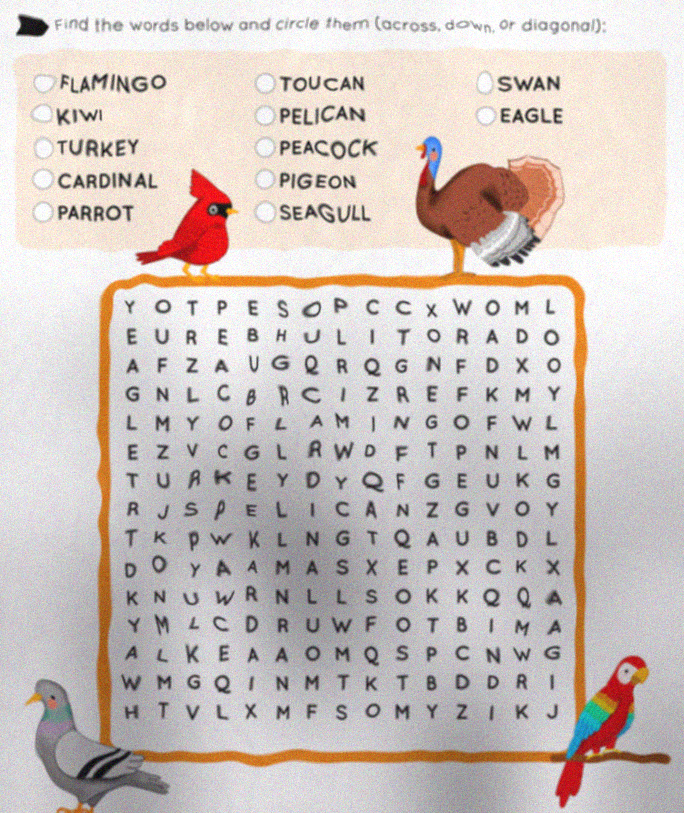
\includegraphics[width=\linewidth]{ressources/image_3.png}
      \caption{Grille avec des éléments autours, froissée et avec des zones d'exposition différentes}
    \endminipage
\end{figure}


\subsection{Chargement des images}

Le chargement des images est réalisé à l'aide de GTK, qui gère le chargement et la manipulation des fichiers image.

La rotation est effectuée à l'aide de la bibliothèque graphique \texttt{cairo}, qui offre des transformations 2D de haute qualité.

\subsection{Extraction de la grille}

Après avoir chargé l'image, on commence par la pré-traitement de l'image pour la rendre plus facile à traiter.

\subsubsection{Transformation en niveaux de gris}
\begin{figure}[!htb]
    \stepimage[0.30\textwidth]{image_1_step_01_grayscale.png}{}
    \stepimage[0.30\textwidth]{image_2_step_01_grayscale.png}{}
    \stepimage[0.26\textwidth]{image_3_step_01_grayscale.png}{}
\end{figure}
On commence par transformer l'image en niveaux de gris pour la rendre plus facile à traiter.
En utilisant la formule de luminance standard :

\[
Y = 0.299 \cdot R + 0.587 \cdot G + 0.114 \cdot B
\]

Où $R$, $G$ et $B$ sont les valeurs des composantes rouge, vert et bleu de l'image.


\subsection{Débruitage adaptatif}
\begin{figure}[!htb]
    \stepimage[0.30\textwidth]{image_1_step_02_adaptive_denoise.png}{}
    \stepimage[0.30\textwidth]{image_2_step_02_adaptive_denoise.png}{}
    \stepimage[0.26\textwidth]{image_3_step_02_adaptive_denoise.png}{}
\end{figure}
Le niveau de bruit est estimé par la variance locale (\(3 \times 3\) pixels) des intensités :
\[
\sigma_{\text{bruit}}^{2} = \frac{1}{|S|} \sum_{s \in S} \frac{1}{N} \sum_{p \in W_s} \big(I(p) - \mu_s\big)^2, \quad \mu_s = \frac{1}{N} \sum_{p \in W_s} I(p)
\]
Cette étape vise à légèrement réduire le bruit pour faciliter les traitements ultérieurs, plutôt qu'à l'éliminer parfaitement.
\newline
Un niveau de bruit normalisé \(\eta = \min(1, \sigma_{\text{bruit}}^{2}/1000)\) ajuste les paramètres du filtre gaussien :
\begin{itemize}
    \item $\eta < 0.1$ : noyau $3\times3$, $\sigma=0.5$
    \item $0.1 \leq \eta < 0.3$ : noyau $3\times3$, $\sigma=1.0$
    \item $\eta \geq 0.3$ : noyau $5\times5$, $\sigma=1.5$
\end{itemize}

\subsection{Seuil adaptatif}
\begin{figure}[!htb]
    \stepimage[0.30\textwidth]{image_1_step_03_threshold.png}{}
    \stepimage[0.30\textwidth]{image_2_step_03_threshold.png}{}
    \stepimage[0.26\textwidth]{image_3_step_03_threshold.png}{}
\end{figure}
Le seuillage adaptatif binarise l'image en calculant un seuil local \(T(x, y)\) pour chaque pixel, basé sur un voisinage de taille \(\texttt{block\_size} \times \texttt{block\_size}\). Deux méthodes sont utilisées :

\subsubsection{Méthode de la moyenne}
Le seuil \(T(x, y)\) est la moyenne des intensités des pixels dans le voisinage \(W_{xy}\), moins une constante \(C\) :
\[
T(x, y) = \frac{1}{N} \sum_{(i, j) \in W_{xy}} I(i, j) - C
\]
Où \(N = \texttt{block\_size}^2\) est le nombre de pixels dans la fenêtre et \(I(i, j)\) est l'intensité du pixel.

\subsubsection{Méthode Gaussienne}
Le seuil est une somme pondérée des intensités du voisinage \(W_{xy}\), où les poids \(w(i, j)\) sont dérivés d'un noyau gaussien et normalisés. Une constante \(C\) est soustraite :
\[
T(x, y) = \sum_{(i, j) \in W_{xy}} w(i, j) \cdot I(i, j) - C
\]

\subsubsection{Application du seuil}
L'image de sortie \(I_{\text{out}}\) est générée en appliquant le seuil \(T(x, y)\) :
\begin{itemize}
    \item \textbf{\texttt{THRESH\_BINARY}}:
    \[
    I_{\text{out}}(x, y) =
    \begin{cases}
    \text{max\_value} & \text{si } I(x, y) > T(x, y) \\
    0 & \text{sinon}
    \end{cases}
    \]
    \item \textbf{\texttt{THRESH\_BINARY\_INV}}:
    \[
    I_{\text{out}}(x, y) =
    \begin{cases}
    0 & \text{si } I(x, y) > T(x, y) \\
    \text{max\_value} & \text{sinon}
    \end{cases}
    \]
\end{itemize}


\subsection{Detection de la grille}
\begin{figure}[!htb]
    \stepimage[0.30\textwidth]{image_1_step_05_grid_extraction.png}{}
    \stepimage[0.30\textwidth]{image_2_step_05_grid_extraction.png}{}
    \stepimage[0.26\textwidth]{image_3_step_05_grid_extraction.png}{}
\end{figure}

Une fois l'image binarisée, l'étape suivante consiste à localiser et à extraire la grille. L'approche est basée sur l'hypothèse que la grille est le plus grand objet de l'image.

\subsubsection{1. Recherche des contours}
Les contours de tous les objets sont identifiés avec un algorithme de suivi de bordure (inspiré de Suzuki \cite{suzuki1985topological}). L'algorithme parcourt l'image à la recherche d'un pixel de départ d'un objet non encore traité. Une fois trouvé, il suit la frontière de l'objet en examinant les 8 pixels voisins (voisinage de Moore) jusqu'à revenir au point de départ. Ce processus est répété pour tous les objets, générant une liste de contours définis par des listes de points.

\subsubsection{2. Identification du plus grand contour}
L'heuristique est que la grille est le plus grand objet. L'aire de chaque contour est calculée, et celui avec la plus grande superficie est sélectionné.

\subsubsection{3. Calcul de la boîte englobante (Bounding Box)}
Un rectangle droit (non incliné) englobant le contour de la grille est calculé pour obtenir ses coordonnées \((x, y)\), sa largeur et sa hauteur, simplifiant ainsi l'extraction.

\subsubsection{4. Extraction de la grille}
Avec la boîte englobante, la région de la grille est rognée de l'image en niveaux de gris. \newline\textcolor{orange}{\HandRight} \textit{Cette première extraction peut être imprécise et sera affinée par un second algorithme.}

\subsection{Nettoyage morphologique de la grille}

\begin{figure}[!htb]
  \stepimage[0.30\textwidth]{image_1_step_07_cleaned_grid.png}{}
  \stepimage[0.30\textwidth]{image_2_step_07_cleaned_grid.png}{}
  \stepimage[0.26\textwidth]{image_3_step_07_cleaned_grid.png}{}
\end{figure}
L'image de la grille extraite peut présenter des imperfections telles que des trous ou des coupures dans les lignes. Pour corriger cela, une opération de \texttt{fermeture morphologique} est appliquée. Elle combine deux processus pour nettoyer l'image \cite{serra1982image}:

\begin{itemize}
    \item \textbf{La dilatation :} Elle épaissit les lignes blanches pour combler les petits trous et reconnecter les segments brisés.
    \newline\textbf{Au niveau du pixel :} Un pixel devient blanc si \textit{au moins un} de ses voisins (défini par un élément structurant 2x2) est blanc. Cela étend les zones blanches.

    \item \textbf{L'érosion :} Opération inverse, elle amincit les lignes pour restaurer leur épaisseur d'origine et éliminer le bruit.
    \newline\textbf{Au niveau du pixel :} Un pixel ne devient blanc que si \textit{tous} ses voisins sont blancs. Cette règle plus stricte supprime les taches de bruit.
\end{itemize}

L'effet net de la fermeture est de nettoyer la grille en éliminant les défauts dans les lignes blanches, tout en préservant la structure globale de la grille.

\subsection{Analyse de la Structure de la Grille}

Après avoir isolé et nettoyé l'image de la grille, l'objectif est de la segmenter en cellules individuelles, chacune contenant une seule lettre. L'approche pour y parvenir dépend de la nature de la grille elle-même : certaines grilles sont dessinées avec des lignes internes séparant chaque cellule, tandis que d'autres ne contiennent que les lettres. Notre algorithme doit donc gérer ces deux cas distincts.
Cette analyse de la structure interne vient ainsi affiner et compléter l'extraction globale de la grille vue précédemment, en nous permettant d'identifier précisément chaque cellule.

\subsubsection{Cas 1 : Grille avec lignes internes (Détection par Lignes)}

\begin{figure}[H]
  \centering
  \minipage{0.30\textwidth}
      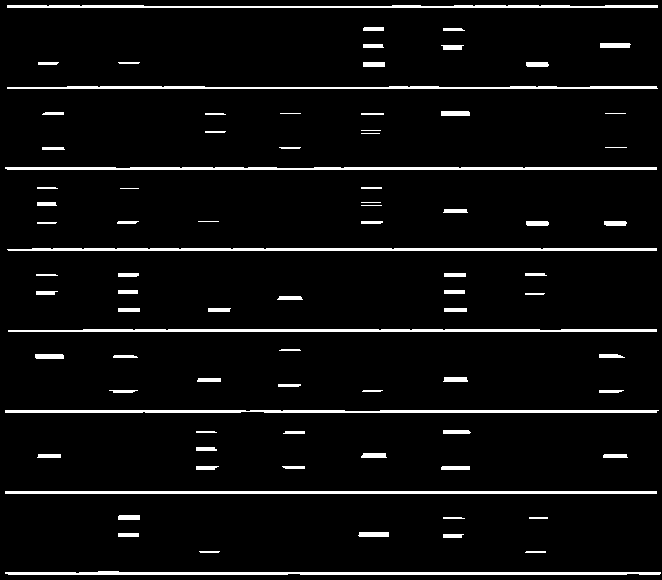
\includegraphics[width=\linewidth]{ressources/image_1_step_09_horizontal_lines.png}
      \caption{}
    \endminipage\quad\quad\quad\quad
    \minipage{0.30\textwidth}
    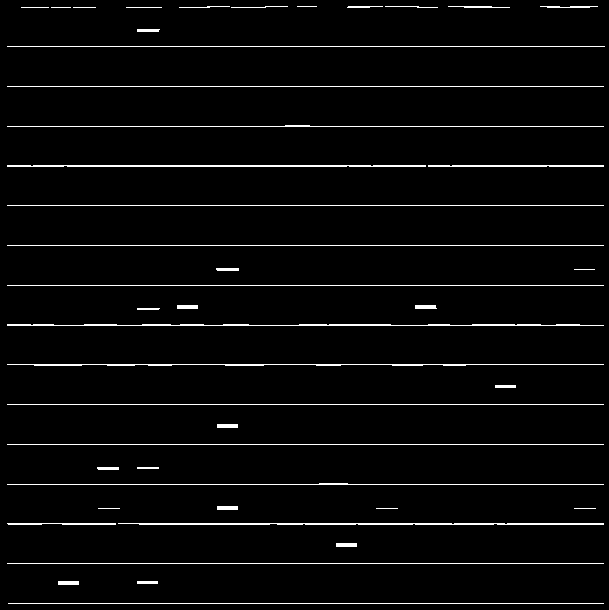
\includegraphics[width=\linewidth]{ressources/image_2_step_09_horizontal_lines.png}
    \caption{}
  \endminipage
  \caption{Détection des lignes horizontales.}
\end{figure}


\begin{figure}[H]
  \centering
  \minipage{0.30\textwidth}
      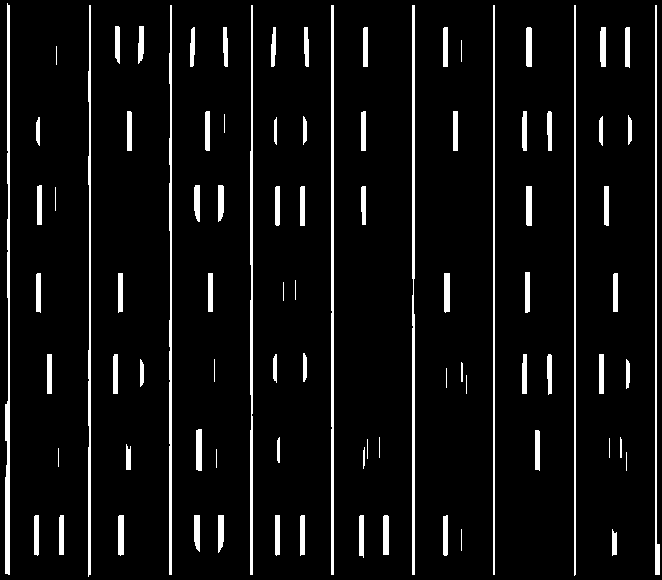
\includegraphics[width=\linewidth]{ressources/image_1_step_09_vertical_lines.png}
      \caption{}
    \endminipage\quad\quad\quad\quad
    \minipage{0.30\textwidth}
    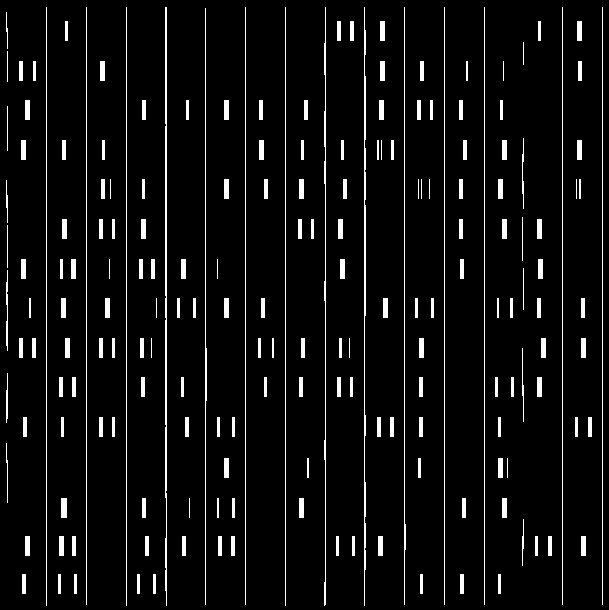
\includegraphics[width=\linewidth]{ressources/image_2_step_09_vertical_lines.png}
    \caption{}
  \endminipage
  \caption{Détection des lignes verticales.}
\end{figure}
Cette méthode est utilisée lorsque l'image de la grille contient des lignes horizontales et verticales clairement visibles qui délimitent les cellules.

\paragraph{1. Détection des lignes}
Pour extraire les lignes, nous utilisons une opération spécialisée appelée \texttt{ouverture morphologique}. Celle-ci est particulièrement efficace pour supprimer les petits objets d'une image tout en préservant la forme et la taille des objets plus grands. L'opération se déroule en deux temps, en utilisant un noyau (ou "élément structurant") adapté à la forme que l'on souhaite conserver. La détection de ligne peut également être fait avec un algorithme de Hough \cite{duda1972use}.

\begin{itemize}
    \item \textbf{Pour les lignes horizontales}, on utilise un élément structurant très large et fin (par exemple, de 40x1 pixels).
    \begin{enumerate}
        \item \textbf{Étape d'érosion :} L'image est d'abord érodée avec ce noyau horizontal. Rappelons que l'érosion amincit les formes. Comme le noyau est très large, tout objet blanc qui est plus fin que 40 pixels horizontalement (comme les lettres, le bruit, ou les lignes verticales) sera complètement "rongé" et disparaîtra. Seules les longues lignes horizontales survivront à cette étape, bien qu'elles soient amincies.
        \item \textbf{Étape de dilatation :} L'image résultante (ne contenant que des lignes horizontales amincies) est ensuite dilatée avec le même noyau. La dilatation épaissit les formes. Cette étape a pour effet de restaurer les lignes horizontales à leur épaisseur d'origine.
    \end{enumerate}
    Le résultat net de cette ouverture est une image ne contenant que les lignes horizontales de la grille.

    \item \textbf{Pour les lignes verticales}, le principe est identique, mais on utilise un élément structurant très haut et étroit (par exemple, 1x40 pixels).
    \begin{enumerate}
        \item \textbf{Étape d'érosion :} L'érosion avec ce noyau vertical supprime tous les objets qui ne sont pas de longues lignes verticales.
        \item \textbf{Étape de dilatation :} La dilatation qui suit restaure l'épaisseur des lignes verticales qui ont survécu.
    \end{enumerate}
\end{itemize}

\paragraph{2. Fusion et Extension des Lignes}
Les lignes détectées par l'ouverture morphologique peuvent être fragmentées. Pour reconstruire des lignes complètes, un traitement supplémentaire est appliqué. Les segments de ligne qui sont colinéaires (sur le même axe) sont identifiés et fusionnés en un seul segment continu. Ensuite, ces segments fusionnés sont étendus sur toute la largeur (pour les lignes horizontales) ou toute la hauteur (pour les lignes verticales) de la grille. Cette étape garantit que la grille est entièrement délimitée, même si certaines parties des lignes étaient manquantes dans l'image nettoyée.

\paragraph{3. Détermination des frontières}
Une fois les images des lignes obtenues, les frontières des cellules sont déterminées en analysant les projections de ces images. On scanne chaque ligne (pour les frontières horizontales) et chaque colonne (pour les frontières verticales) pour identifier les positions exactes des lignes détectées. Ces positions deviennent les délimitations des cellules.

\subsubsection{Cas 2 : Grille sans lignes internes (Détection par Lettres)}

\begin{figure}[H]
  \centering
  \minipage{0.30\textwidth}
      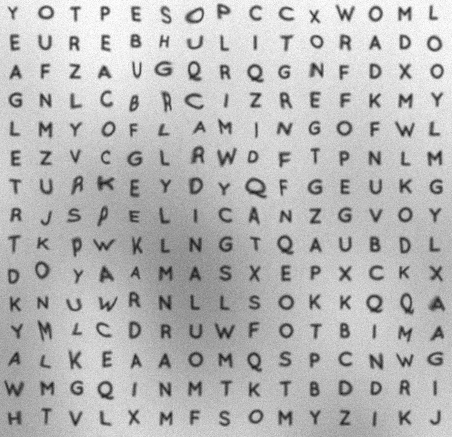
\includegraphics[width=\linewidth]{ressources/image_3_step_08_text_region.png}
      \caption{}
    \endminipage\hfill
\end{figure}
Lorsque la grille ne contient pas de lignes internes, nous devons déduire sa structure en nous basant sur la disposition des lettres elles-mêmes.

\paragraph{1. Localisation de la région de texte}
D'abord, nous détectons tous les contours dans l'image de la grille et nous les filtrons pour ne garder que ceux qui ressemblent à des lettres (en se basant sur leur taille, leur forme, etc.). Ensuite, nous calculons la boîte englobante de l'ensemble de ces contours de lettres. Cette boîte définit la "région de texte", qui est une version plus précise de la grille, débarrassée des marges vides.


\paragraph{2. Inférence des dimensions de la grille}
Pour déduire le nombre de lignes et de colonnes à partir des positions des lettres, un algorithme de clustering est utilisé. L'idée est de regrouper les lettres qui sont alignées. L'algorithme traite les coordonnées Y et X des centres des lettres de manière indépendante. D'abord, il groupe les coordonnées Y qui sont très proches pour déterminer le nombre de lignes distinctes. Ensuite, il répète le processus sur les coordonnées X pour trouver le nombre de colonnes. Le nombre de groupes finaux pour chaque axe nous donne les dimensions de la grille.

\paragraph{3. Création d'une grille virtuelle}
Connaissant les dimensions de la région de texte et le nombre de lignes et de colonnes, nous pouvons générer une grille virtuelle en divisant simplement la région en cellules de taille égale.

\subsubsection{Résultat : La grille segmentée}

Quelle que soit la méthode utilisée, le résultat final est une série de coordonnées qui définissent les frontières de chaque cellule de la grille. Cela nous permet de "découper" chaque lettre individuellement pour la reconnaissance de caractères.

\begin{figure}[H]
    \stepimage[0.30\textwidth]{image_1_step_10_reconstructed_grid.png}{}
    \stepimage[0.30\textwidth]{image_2_step_10_reconstructed_grid.png}{}
    \stepimage[0.26\textwidth]{image_3_step_10_reconstructed_grid.png}{}
    \caption{Grille segmentée avec les frontières des cellules détectées.}
\end{figure}

\section{Extraction de la Liste de Mots}
L'étape finale consiste à extraire la liste des mots à rechercher à partir d'une région de l'image. Ce processus est une chaîne de traitement d'image à part entière, conçue pour isoler des lignes de texte.

\subsection{Pré-traitement et Binarisation}
\paragraph{1. Préparation de l'image}
Comme pour la grille, l'image est d'abord convertie en niveaux de gris et un léger flou gaussien est appliqué pour réduire le bruit et lisser les caractères.

\paragraph{2. Binarisation par Combinaison}
Le texte peut être difficile à segmenter à cause des variations d'éclairage, des ombres ou de la qualité de l'impression. Pour surmonter cela, au lieu d'une seule méthode de seuillage, nous en combinons deux pour maximiser nos chances de capturer tout le texte :

  \begin{itemize}
    \item \textbf{Méthode d'Otsu \cite{otsu1979threshold} :} La méthode d'Otsu est un algorithme de seuillage automatique qui analyse l'histogramme des intensités de l'image pour trouver le seuil optimal. Ce seuil est la valeur qui maximise la variance entre les deux classes de pixels (premier-plan et arrière-plan) qu'elle sépare. Elle est particulièrement efficace pour les images à contraste élevé, comme du texte noir sur fond blanc.
    \begin{figure}[H]
      \centering
      \minipage{0.29\textwidth}
          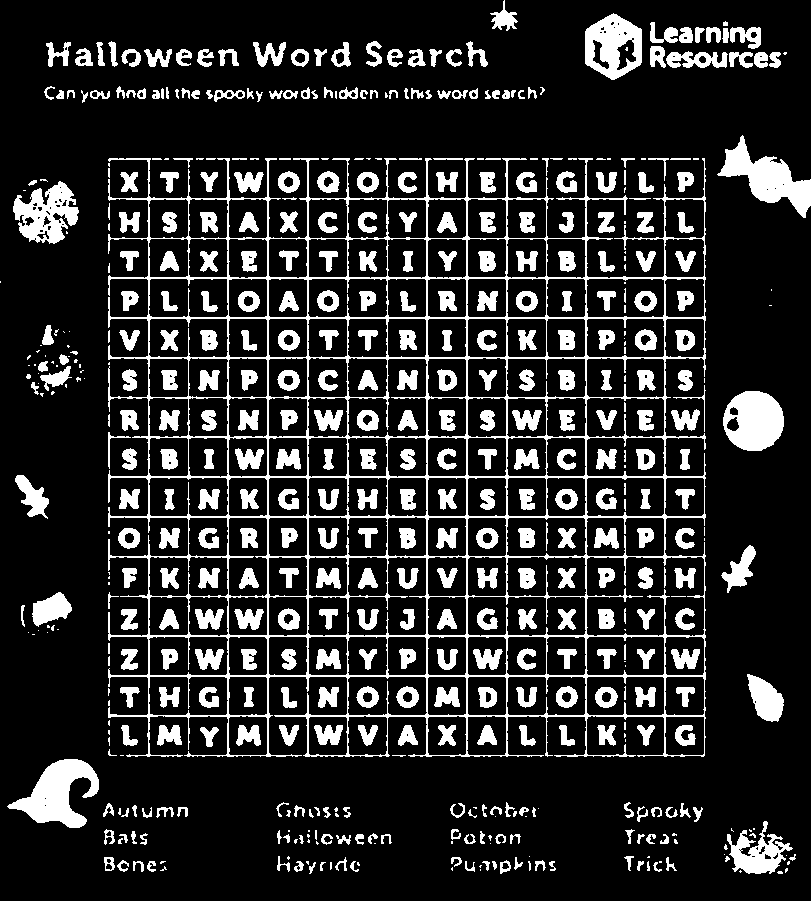
\includegraphics[width=\linewidth]{ressources/image_2_word_detection_03_otsu_threshold.png}
          \caption{}
        \endminipage\quad\quad\quad\quad
        \minipage{0.25\textwidth}
        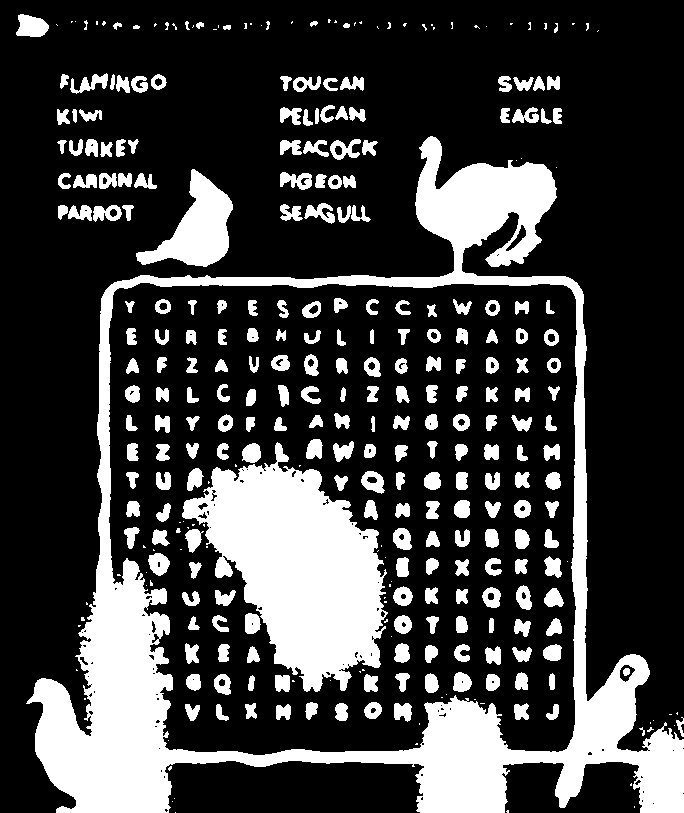
\includegraphics[width=\linewidth]{ressources/image_3_word_detection_03_otsu_threshold.png}
        \caption{}
      \endminipage
      \caption{Seuillage par Otsu.}
    \end{figure}

    \item \textbf{Seuillage par la Moyenne :} Une version plus simple du seuillage global, où le seuil est calculé comme un pourcentage (par exemple, 80\%) de l'intensité moyenne de tous les pixels de l'image.
    \begin{figure}[H]
      \centering
      \minipage{0.29\textwidth}
          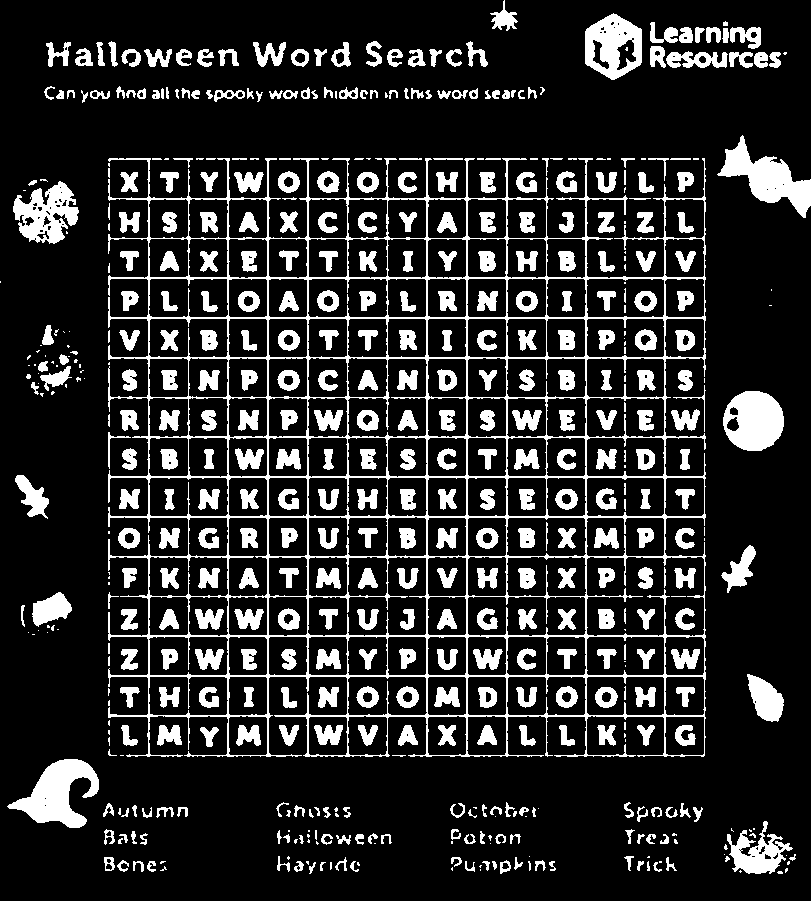
\includegraphics[width=\linewidth]{ressources/image_2_word_detection_05_mean_threshold.png}
          \caption{}
        \endminipage\quad\quad\quad\quad
        \minipage{0.25\textwidth}
        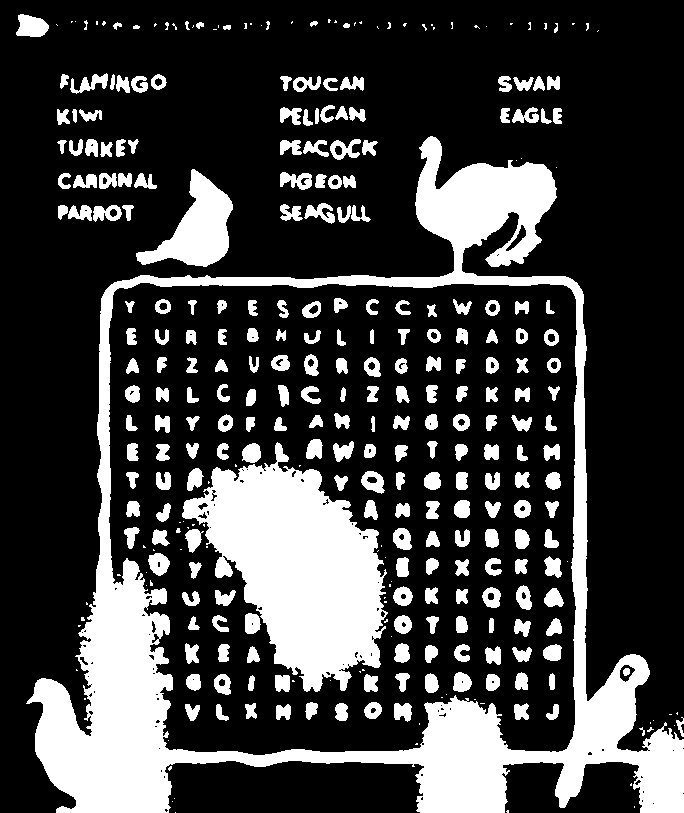
\includegraphics[width=\linewidth]{ressources/image_3_word_detection_05_mean_threshold.png}
        \caption{}
      \endminipage
      \caption{Seuillage par la moyenne.}
    \end{figure}
\end{itemize}

\paragraph{3. Fusion des Résultats}
Les deux images binaires résultantes sont ensuite fusionnées en une seule image en utilisant une opération \texttt{OU} logique pixel à pixel. Un pixel est considéré comme faisant partie du texte dans l'image finale s'il a été classé comme tel par \textit{au moins une} des deux méthodes.
\begin{figure}[H]
  \centering
  \minipage{0.29\textwidth}
      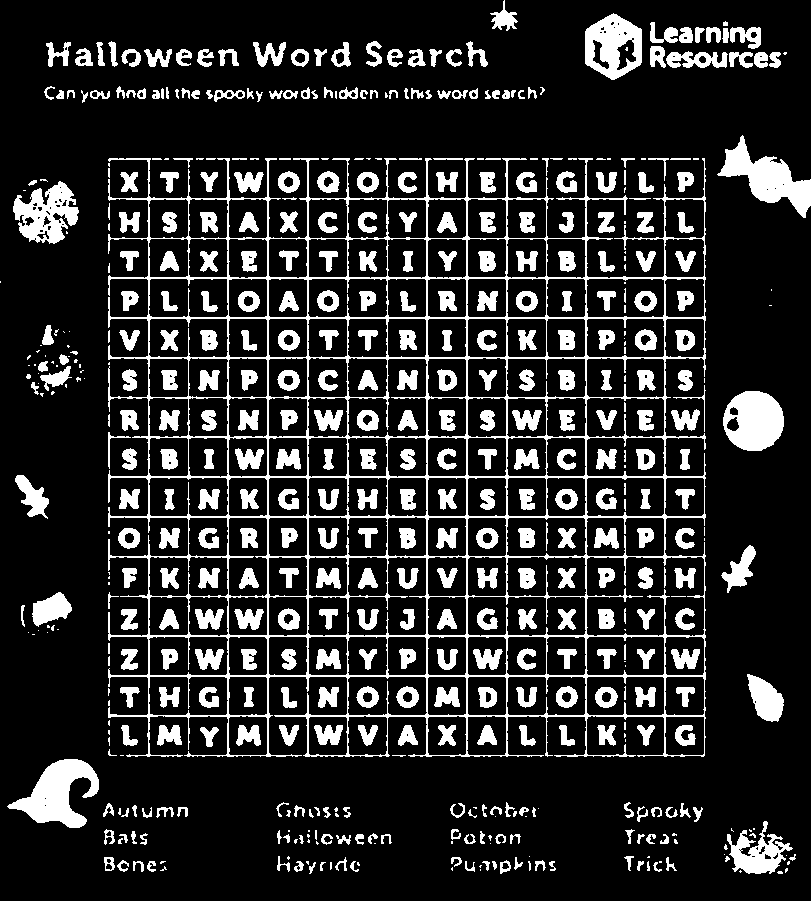
\includegraphics[width=\linewidth]{ressources/image_2_word_detection_06_combined_threshold.png}
      \caption{}
    \endminipage\quad\quad\quad\quad
    \minipage{0.25\textwidth}
    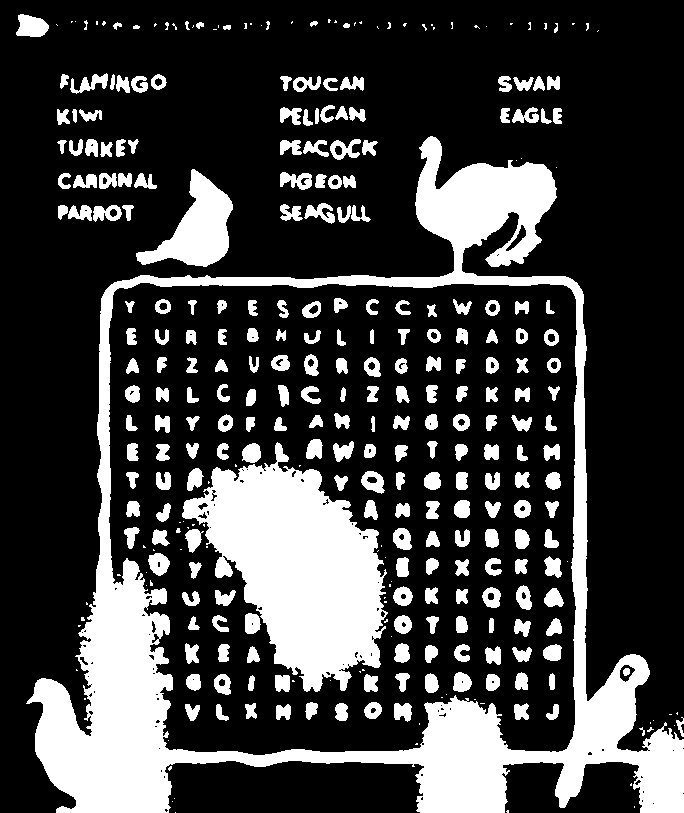
\includegraphics[width=\linewidth]{ressources/image_3_word_detection_06_combined_threshold.png}
    \caption{}
  \endminipage
  \caption{Fusion des résultats.}
\end{figure}
\subsection{Analyse et Groupement des Mots}
Une fois l'image binarisée, des opérations morphologiques sont appliquées pour transformer les lettres individuelles en des "blobs" solides correspondant à des mots entiers. Une séquence de \texttt{fermeture}, de \texttt{dilatation} et d'\texttt{érosion} permet de combler les trous dans les lettres et de connecter les caractères adjacents.

\begin{figure}[H]
  \centering
  \minipage{0.29\textwidth}
      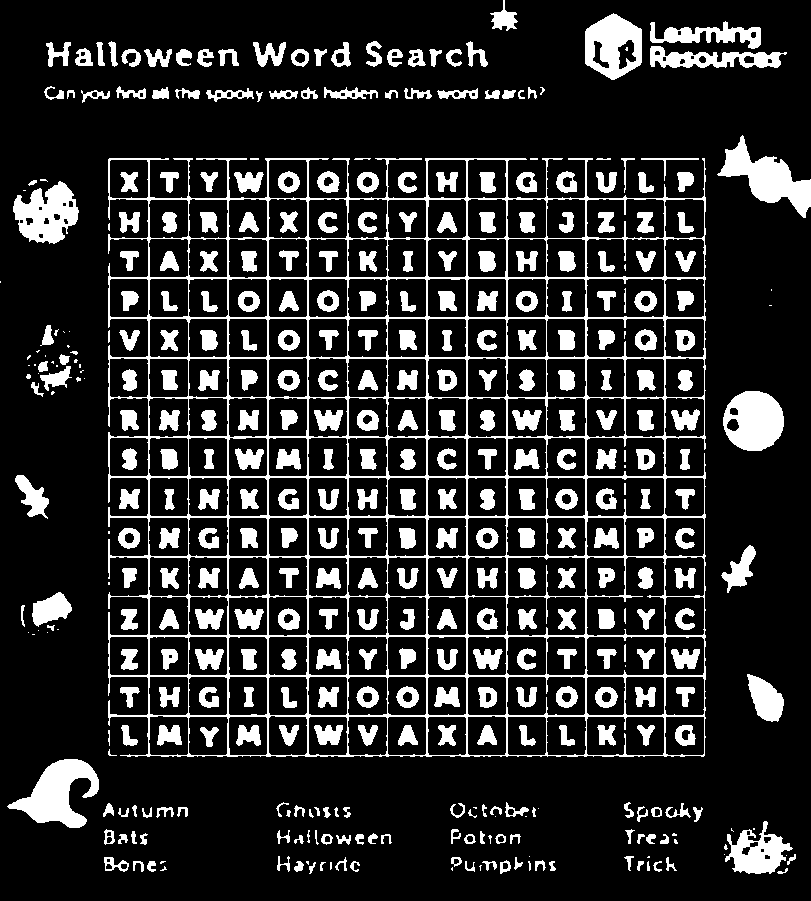
\includegraphics[width=\linewidth]{ressources/image_2_word_detection_07_morphology_closed.png}
      \caption{}
    \endminipage\quad\quad\quad\quad
    \minipage{0.25\textwidth}
    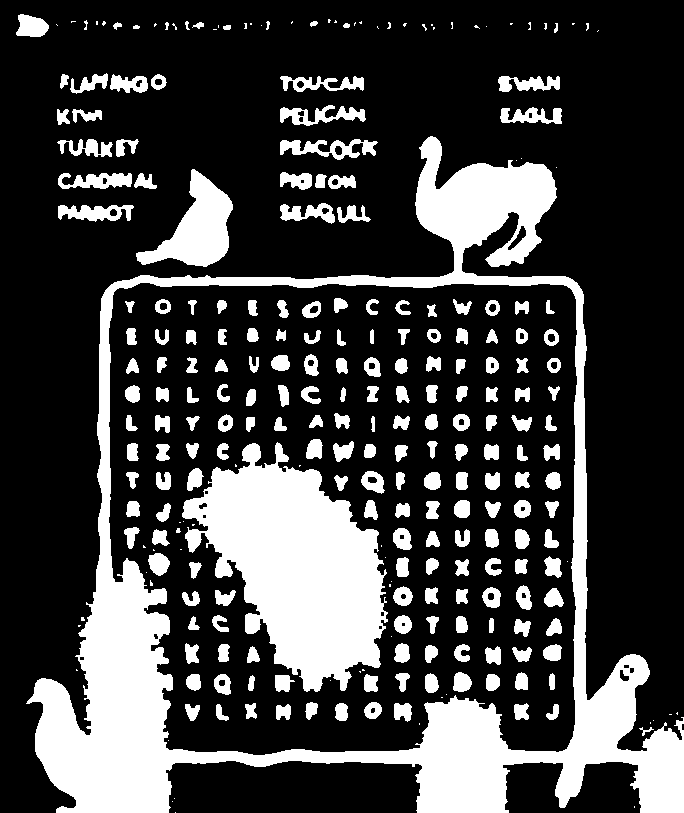
\includegraphics[width=\linewidth]{ressources/image_3_word_detection_07_morphology_closed.png}
    \caption{}
  \endminipage
  \caption{Fermeture morphologique.}
\end{figure}
\begin{figure}[H]
  \centering
  \minipage{0.29\textwidth}
      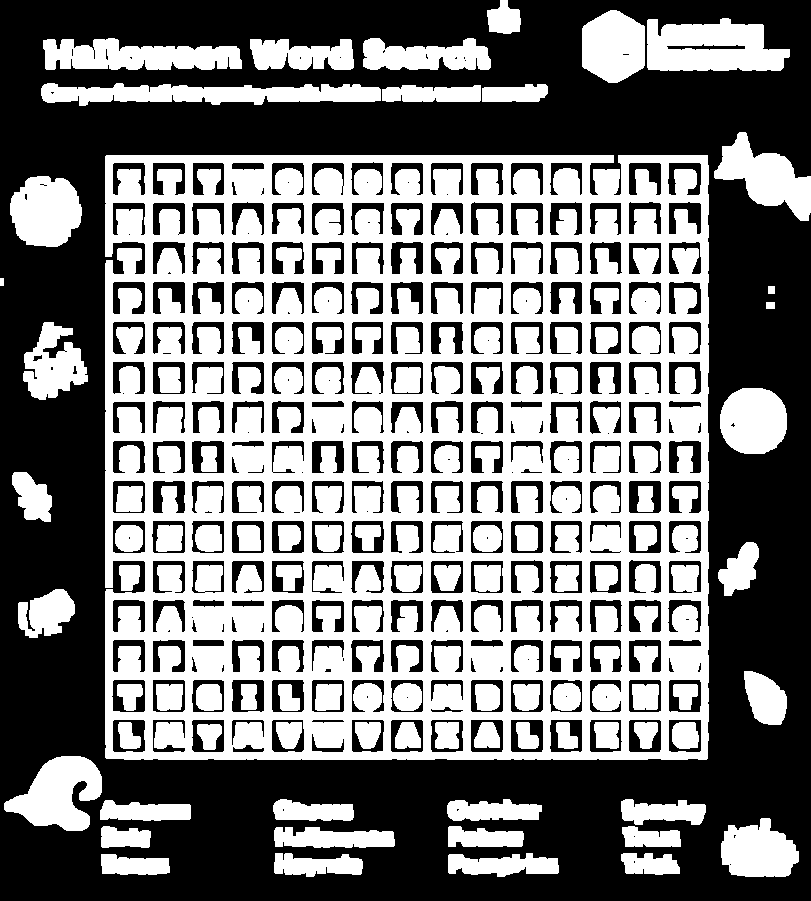
\includegraphics[width=\linewidth]{ressources/image_2_word_detection_08_dilated.png}
      \caption{}
    \endminipage\quad\quad\quad\quad
    \minipage{0.25\textwidth}
    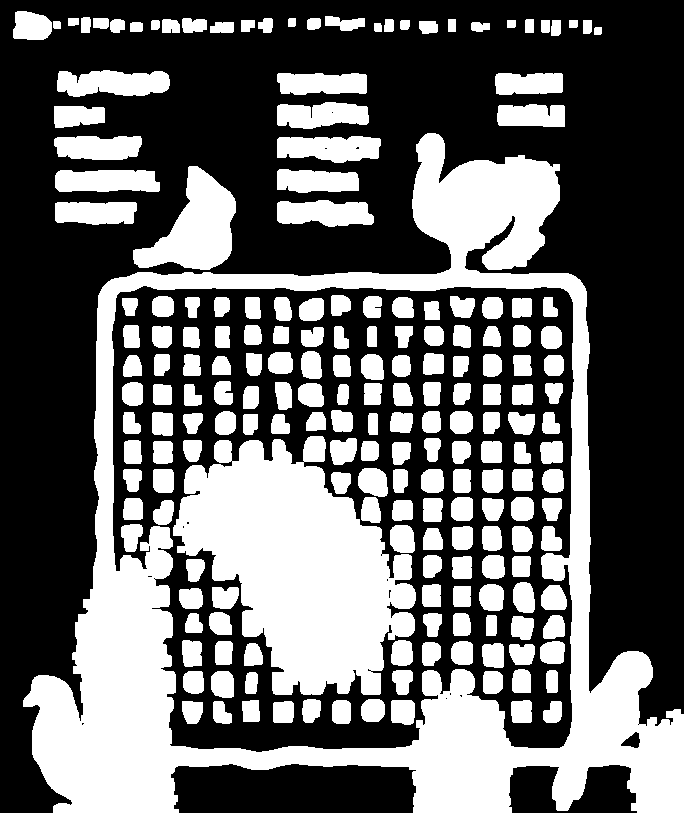
\includegraphics[width=\linewidth]{ressources/image_3_word_detection_08_dilated.png}
    \caption{}
  \endminipage
  \caption{Dilatation.}
\end{figure}
\begin{figure}[H]
  \centering
  \minipage{0.29\textwidth}
      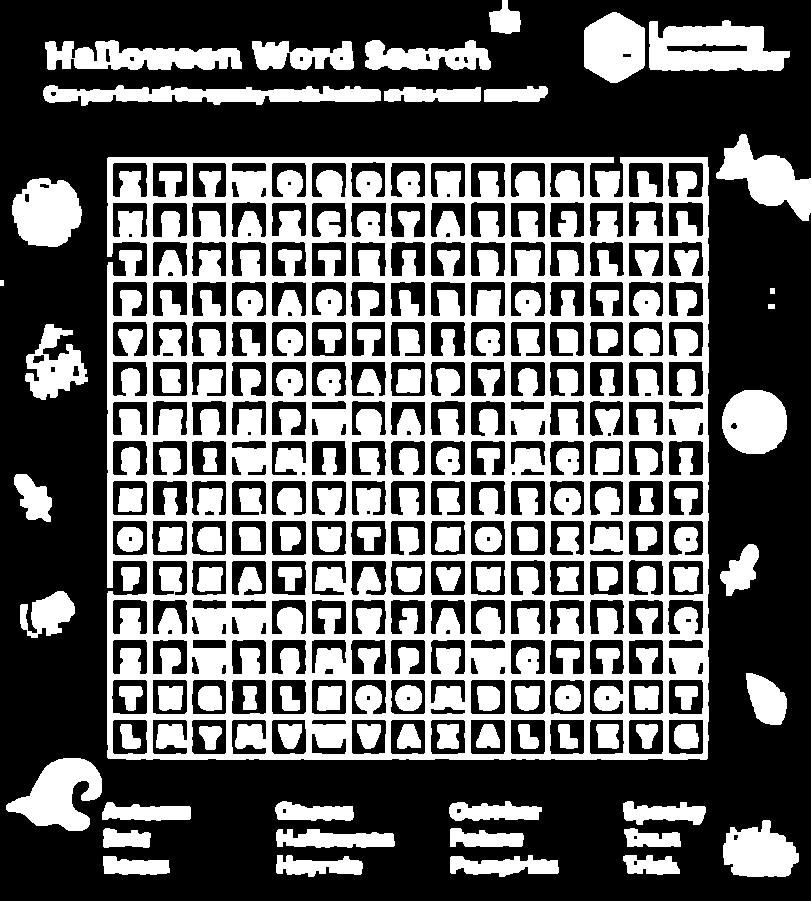
\includegraphics[width=\linewidth]{ressources/image_2_word_detection_09_eroded.png}
      \caption{}
    \endminipage\quad\quad\quad\quad
    \minipage{0.25\textwidth}
    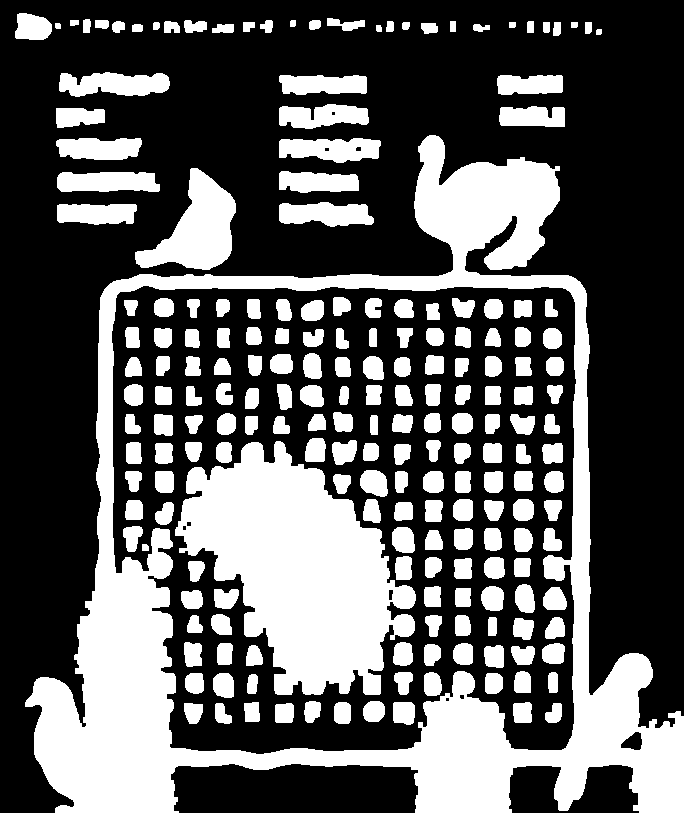
\includegraphics[width=\linewidth]{ressources/image_3_word_detection_09_eroded.png}
    \caption{}
  \endminipage
  \caption{Érosion.}
\end{figure}
\paragraph{1. Détection et Filtrage :} Comme précédemment, les contours de tous les "blobs" sont détectés, et ceux qui ne correspondent pas à des critères géométriques de mots (taille, ratio, etc.) sont éliminés.

\paragraph{2. Fusion Horizontale des Mots :} Pour regrouper les fragments de mots, un algorithme de fusion est appliqué. Après avoir trié les boîtes englobantes des contours par leur coordonnée X, l'algorithme les parcourt. Si une boîte est suffisamment proche horizontalement et alignée verticalement avec la précédente, elles sont fusionnées. Sinon, la boîte précédente est considérée comme un mot complet. Ce processus garantit que seuls les fragments de mots adjacents et colinéaires sont assemblés.

\paragraph{3. Identification de la Liste de Mots :} Pour identifier la liste de mots principale, les mots sont d'abord regroupés en lignes par clustering vertical de leurs centres. Ensuite, l'algorithme analyse l'espacement vertical entre les lignes pour identifier l'interligne le plus courant. En se basant sur cet interligne, il regroupe les lignes en blocs. Finalement, le bloc contenant le plus grand nombre de mots est sélectionné comme étant la liste de mots à rechercher. Le résultat est un ensemble final de boîtes englobantes, chacune correspondant à un mot à trouver.

\begin{figure}[H]
  \centering
  \minipage{0.29\textwidth}
      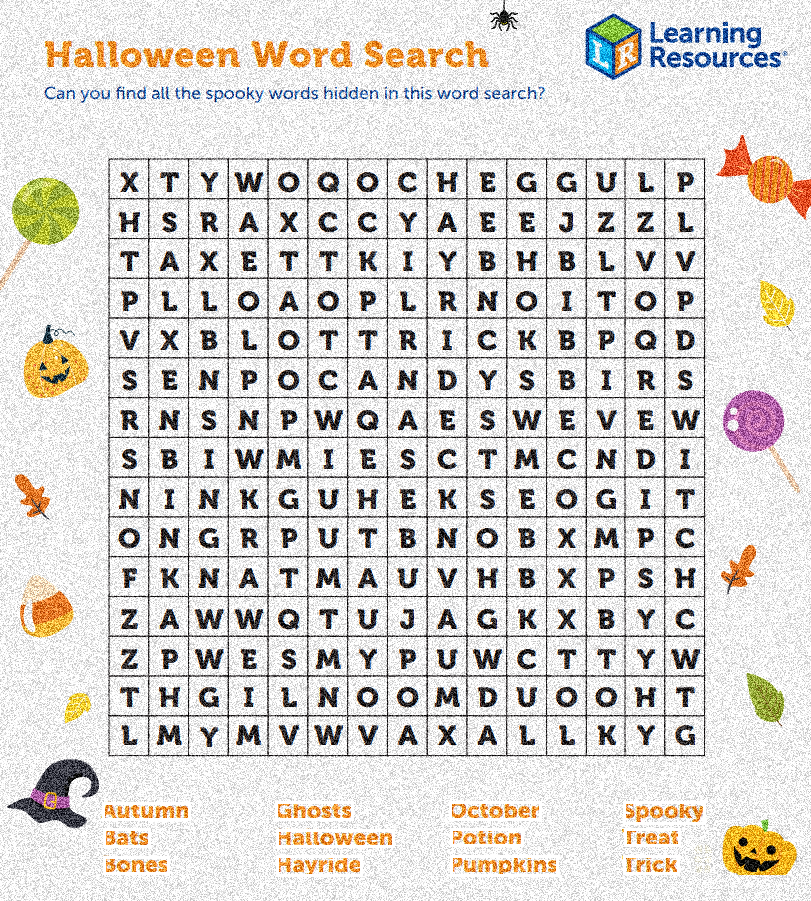
\includegraphics[width=\linewidth]{ressources/image_2_word_detection_10_detected_words.png}
      \caption{}
    \endminipage\quad\quad\quad\quad
    \minipage{0.25\textwidth}
    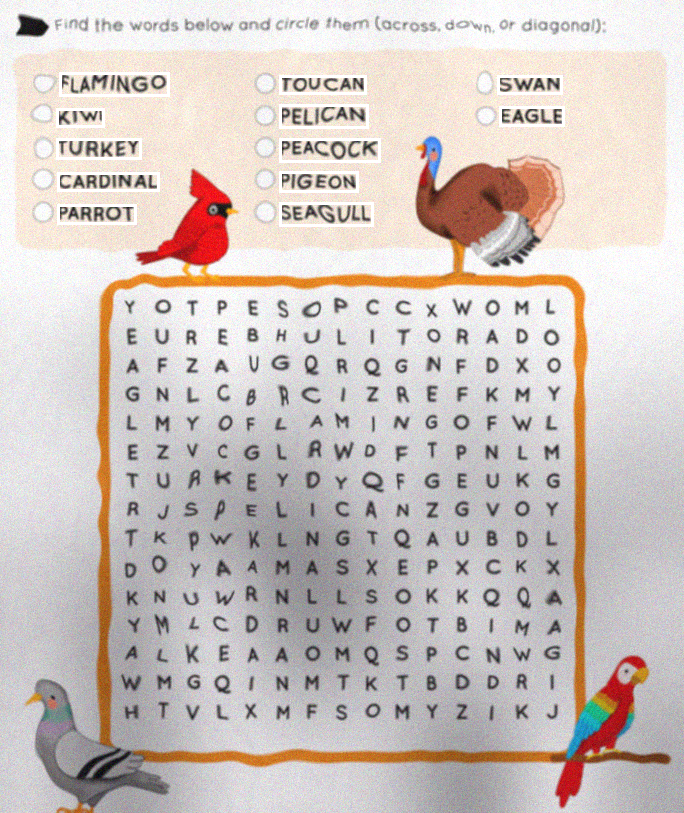
\includegraphics[width=\linewidth]{ressources/image_3_word_detection_10_detected_words.png}
    \caption{}
  \endminipage
  \caption{Détection des mots.}
\end{figure}

\section{Réseau de Neurones pour la fonction XNOR}

Pour démontrer les principes des réseaux de neurones, un simple réseau a été implémenté en C pour apprendre la fonction logique XNOR.

\subsection{Architecture du réseau}

Le réseau possède une architecture de type \textit{feed-forward} composée de trois couches :

\begin{itemize}
    \item \textbf{Couche d'entrée :} Elle est composée de 2 neurones, qui correspondent aux deux entrées binaires de la fonction XNOR.
    \item \textbf{Couche cachée :} Elle contient 2 neurones. Chaque neurone est entièrement connecté aux neurones de la couche d'entrée.
    \item \textbf{Couche de sortie :} Elle est constituée d'un seul neurone, qui fournit le résultat final de l'opération XNOR.
\end{itemize}

Tous les neurones du réseau (ceux de la couche cachée et de la couche de sortie) utilisent la fonction d'activation sigmoïde :
\[
f(x) = \frac{1}{1 + e^{-x}}
\]
Cette fonction a pour caractéristique de borner les sorties des neurones entre 0 et 1, ce qui est adapté pour des problèmes de classification binaire. Sa dérivée, utilisée lors de la rétropropagation de l'erreur, est simple à calculer :
\[
f'(x) = f(x) \cdot (1 - f(x))
\]

\subsection{Apprentissage par Rétropropagation}

L'entraînement du réseau est réalisé grâce à l'algorithme de rétropropagation du gradient (\textit{backpropagation}).

\begin{itemize}
    \item \textbf{Initialisation :} Les poids des connexions et les biais des neurones sont initialisés avec des valeurs aléatoires.
    \item \textbf{Propagation avant (\textit{Forward Propagation}) :} Pour chaque exemple d'entraînement, les entrées sont propagées à travers le réseau, de la couche d'entrée à la couche de sortie, pour calculer une prédiction.
    \item \textbf{Calcul de l'erreur :} L'erreur entre la sortie prédite et la sortie attendue est calculée (par exemple, avec l'erreur quadratique moyenne).
    \item \textbf{Rétropropagation de l'erreur :} L'erreur est ensuite propagée en sens inverse, de la couche de sortie vers la couche d'entrée. À chaque couche, on calcule le gradient de l'erreur par rapport aux poids et aux biais.
    \item \textbf{Mise à jour des poids :} Les poids et les biais du réseau sont ajustés dans la direction opposée du gradient, afin de minimiser l'erreur. Cette mise à jour est pondérée par un \textit{taux d'apprentissage} (learning rate).
\end{itemize}

Les hyperparamètres utilisés pour l'entraînement étaient les suivants :
\begin{itemize}
    \item Taux d'apprentissage : 0.5
    \item Nombre d'époques : 100 000
\end{itemize}

\subsection{Résultats et Performance}

Après 100 000 époques d'entraînement, le réseau est capable de prédire la sortie de la fonction XNOR avec une précision parfaite pour les quatre combinaisons d'entrées possibles. Le temps d'exécution total pour l'entraînement était de \textbf{22.727 ms}.

\begin{table}[H]
    \centering
    \begin{tabular}{|c|c|c|c|c|}
        \hline
        \multicolumn{2}{|c|}{\textbf{Input}} & \textbf{Output Attendu} & \textbf{Output Prédit} & \textbf{Sortie brute du réseau} \\ \hline
        0 & 0 & 1 & 1 & 0.992813 \\ \hline
        0 & 1 & 0 & 0 & 0.006186 \\ \hline
        1 & 0 & 0 & 0 & 0.006188 \\ \hline
        1 & 1 & 1 & 1 & 0.992620 \\ \hline
    \end{tabular}
    \caption{Résultats de prédiction pour la fonction XNOR après entraînement.}
\end{table}

La performance du modèle est la suivante :
\begin{itemize}
    \item \textbf{Précision (Accuracy) :} 4/4 (100.0\%)
    \item \textbf{Erreur Quadratique Moyenne (MSE) :} 0.000046
\end{itemize}
\[
\text{MSE} = \frac{1}{n} \sum_{i=1}^{n} (y_i - \hat{y}_i)^2
\]
Où \(n\) est le nombre d'exemples (4 dans ce cas), \(y_i\) est la sortie attendue et \(\hat{y}_i\) est la prédiction du réseau.

\section{Solver}
Le programme solver a pour but de renvoyer les coordonnées auxquelles se situe le mot recherché dans une grille.

Il prend deux arguments en entrée :
\begin{itemize}
    \item Le nom d’un fichier texte : ce fichier doit contenir une grille de caractères en majuscules et comporter au minimum cinq lignes et cinq colonnes.
    \item Le mot à chercher dans la grille (en majuscules ou en minuscules).
\end{itemize}

Le programme affiche sur la sortie standard :
\begin{itemize}
    \item ``Not Found'' si le mot n’a pas été trouvé ;
    \item (x0,y0)(x1,y1) si le mot a été trouvé, avec :
    \begin{itemize}
        \item (x0, y0) = abscisse et ordonnée (en caractères) de la première lettre du mot dans la grille ;
        \item (x1, y1) = abscisse et ordonnée (en caractères) de la dernière lettre du mot dans la grille.
    \end{itemize}
\end{itemize}

Les coordonnées (0,0) correspondent au premier caractère de la grille (en haut à gauche).

\subsection{Fichiers utilisés}

Le programme solver nécessite l’utilisation de cinq fichiers :
\begin{itemize}
    \item \texttt{main.c}
    \item \texttt{solver.c}
    \item \texttt{solver.h}
    \item \texttt{search.c}
    \item \texttt{search.h}
\end{itemize}

\subsection{main.c}

Le fichier \texttt{main.c} constitue la base du programme.
Il prend les deux arguments cités précédemment en entrée, lit le fichier texte, puis stocke la grille sous forme d’un tableau de tableaux de caractères.

Ensuite, il vérifie la validité du mot à chercher et convertit toutes ses lettres en majuscules.
Enfin, il appelle la fonction \texttt{solver()}.

\subsection{solver.c}

Le fichier \texttt{solver.c} parcourt la grille à la recherche de la première lettre du mot recherché.
Lorsqu’elle est trouvée, il appelle les fonctions de recherche présentes dans \texttt{search.c} :

\begin{itemize}
    \item \texttt{north\_search} : recherche le mot dans la direction Nord ;
    \item \texttt{south\_search} : recherche le mot dans la direction Sud ;
    \item \texttt{east\_search} : recherche le mot dans la direction Est ;
    \item \texttt{west\_search} : recherche le mot dans la direction Ouest ;
    \item \texttt{northeast\_search} : recherche le mot dans la direction Nord-Est ;
    \item \texttt{northwest\_search} : recherche le mot dans la direction Nord-Ouest ;
    \item \texttt{southeast\_search} : recherche le mot dans la direction Sud-Est ;
    \item \texttt{southwest\_search} : recherche le mot dans la direction Sud-Ouest.
\end{itemize}

Si le mot est trouvé, la fonction renvoie ses coordonnées.
Sinon, elle renvoie ``Not Found''.


\newpage
\section*{Bibliographie}
\nocite{*}
\bibliographystyle{plain}
\bibliography{bibliography}

\end{document}
